\chapter{Methods}\label{chap:methods}

\section{Technologies}
The SafeScript project utilizes a comprehensive stack of technologies to deliver a robust and efficient solution for identifying and addressing security 
vulnerabilities in software projects. 
The key technologies employed in this project include:

\begin{itemize}
\item \textbf{Django Framework}: A high-level Python web framework that encourages rapid development and clean, pragmatic design. \cite{django} 
\item \textbf{Python}: The primary programming language used for developing the backend logic and machine learning models. \cite{python}
\item \textbf{SQLite v3}: A lightweight, disk-based database used for storing user credentials, project details, and scanning results. \cite{sqlite} 
\item \textbf{JavaScript}: Used for adding interactive elements to the web pages and handling client-side logic. \cite{javascript} 
\item \textbf{HTML}: The standard markup language for creating web pages. \cite{html} 
\item \textbf{CSS}: A style sheet language used for describing the presentation of the web pages. \cite{css} 
\item \textbf{Bootstrap}: A front-end framework used for developing responsive and mobile-first web pages. \cite{bootstrap} 
\item \textbf{Ajax}: A set of web development techniques used to create asynchronous web applications. \cite{ajax} 
\item \textbf{jQuery}: A fast, small, and feature-rich JavaScript library used to simplify HTML DOM tree traversal and manipulation. \cite{jquery}
\item \textbf{GitPython}: A Python library used to interact with Git repositories.  \cite{gitpython}
\end{itemize}

\section{Implementation}
The implementation of the SafeScript project involves several key components and workflows designed to ensure seamless operation and 
effective vulnerability detection.

\subsection{User Options}
Users are provided with two primary options for submitting their code for analysis:
\begin{enumerate}
\item{\textbf{Single File Import}} Users can upload a single Python source file.
\item{\textbf{Repository Cloning}} Users can provide a link to a code repository (e.g., GitHub, Bitbucket), which the system will clone and analyze.
\end{enumerate}
\subsection{Core Functionalities}
The core functionalities of the system as follows:

\begin{enumerate}

\item{\textbf{User Authentication}}: Users authenticate themselves using a username and password to access the system.
\item{\textbf{Project Creation and Management}}: Users create and manage projects, selecting either to import a single file or clone an entire repository.
\item{\textbf{Code Retrieval}}: The system fetches the code from the specified source.
\item{\textbf{Model Selection}} During the vulnerability detection phase, users can choose between the ChatGPT API and the LSTM model. 
This flexibility allows users to leverage the strengths of both models, ensuring robust and reliable security analysis.
\item{\textbf{Data Conversion}}: The retrieved code is converted into word2vec (w2v) format, preparing it for vulnerability analysis.
\item{\textbf{Vulnerability Detection}}: Users can select either the integrated ChatGPT API or the LSTM model for vulnerability detection.
\item{\textbf{Report Generation}}: The system generates detailed reports outlining detected vulnerabilities, their severity, and recommendations for fixes.
\item{\textbf{Rescan Capability}}: Users can rescan their code after making fixes to ensure that vulnerabilities have been addressed.

\end{enumerate}

\subsection{Frontend and Backend Integration}
The frontend, built with HTML, CSS, Bootstrap, and JavaScript (including jQuery and Ajax), provides a user-friendly interface for interaction. 
The backend, developed using Django, handles the business logic, user authentication, project management, code retrieval, data conversion, 
vulnerability detection, and report generation. 
SQLite v3 is used for database management, ensuring efficient data storage and retrieval.

\subsection{AI Integration}
The AI integration in the SafeScript project leverages advanced machine learning models to enhance the accuracy and efficiency of vulnerability detection. 
At the moment the system is integrated with GPT API and LSTM model, which we have trained over past labs. 
Beside, those two the models have the capability to be integrated with other AI models as well.

\subsubsection{Integrated ChatGPT API}
The system integrates the ChatGPT API, enabling it to utilize the powerful capabilities of the ChatGPT model for analyzing code and 
identifying potential security vulnerabilities. 
This integration allows the system to provide context-aware analysis and generate comprehensive vulnerability reports.
This integration allows the user to detect deffirent types of vulnerabilities in their python code.

\subsubsection{LSTM Model}
In addition to the ChatGPT API, the system incorporates an in-house developed LSTM (Long Short-Term Memory) model. 
This model is specifically trained to detect security vulnerabilities in Python code. 
Users have the option to select the LSTM model for vulnerability detection, benefiting from its specialized focus and accuracy.
The LSTM model for has the capability to detect for specific type of vulnerabilities. The system can detect Cross-Site Scripting (XSS), 
Path Disclosure, Remote Code Execution, Command Injection.
The system has the capability to support more vulnerabilities types through LSTM model in the future.

By integrating these AI technologies, the SafeScript project enhances its capability to detect and report vulnerabilities effectively, 
providing users with actionable insights to improve the security of their software projects.

\section{Data Storage} 

The database for the Vulnerability Scanner project is structured using SQLite v3, providing a lightweight, disk-based database engine. 
This database includes several tables designed to handle user authentication, project management, and feedback functionalities.

The auth\_group table manages the different user groups within the system, facilitating role-based access control. 
The auth\_user table stores user information, including login credentials and profile details, to support user authentication and management. 
The auth\_user\_groups table links users to the groups they belong to, enabling group-based permissions and access control. 
Similarly, the auth\_user\_user\_permissions table maps individual users to specific permissions, allowing for fine-grained access control. 
The auth\_permission table defines various permissions that can be assigned to users or groups, ensuring secure and controlled access 
to different system functionalities.

The django\_admin\_log table records administrative actions performed within the system, providing an audit trail for monitoring and security purposes. 
The django\_content\_type table is used by the Django framework to keep track of all the models installed in the project, 
facilitating content type management. 
The authtoken\_token table stores authentication tokens for users, supporting secure API access.

For project-specific data, the main\_feedback table collects user feedback, including the subject and body of 
feedback messages, along with timestamps and user associations. 
The main\_price table manages pricing information related to the system's services or products, along with 
timestamps for creation and updates. The main\_response table records responses generated by the system, 
including response type, token usage, timestamps, and associated user and request information. 
The main\_log table logs user interactions with the system, capturing details such as user identity, 
URL accessed, user agent, IP address, request method, status code, and timestamps. Lastly, the main\_project 
table manages project information, including project identifiers, names, descriptions, repository details, status, 
timestamps, and associated user information.

These tables collectively support the core functionalities of the Vulnerability Scanner project, including user 
authentication, project management, feedback collection, and logging of interactions and administrative actions. 
This structured approach ensures efficient data management and retrieval, facilitating seamless operation and robust security.
Figure \ref{fig:dataStorage} shows the data storage in Sqlite database.

\begin{figure}[H]
    \centering
    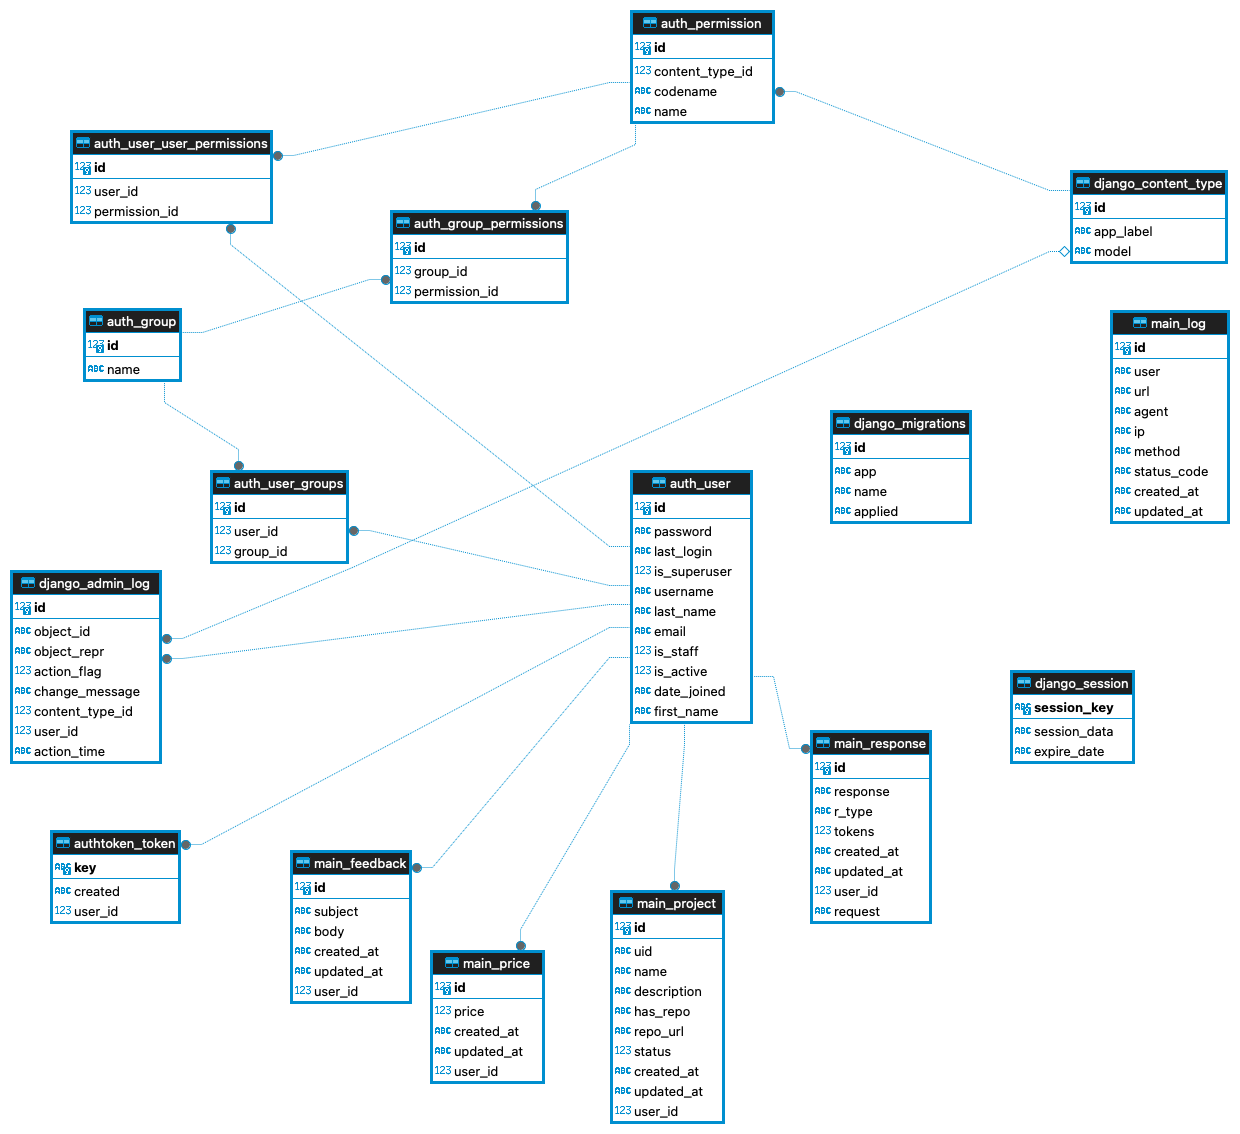
\includegraphics[width=0.9\linewidth]{images/ERD.png}
    \caption{System storage ER diagram}
    \label{fig:dataStorage}
\end{figure}